% Workstream xs appendix: coverage and supplementary tables.
% Tables are generated by `python -m albert.research.flb_xs run latex` from data/research/flb_xs/.

\subsection{Coverage}\label{app:xs-coverage}

\begin{table}[htbp]
\centering
\begin{threeparttable}
\caption{Sampling frame, sample and coverage by group}\label{tab:xs-coverage}
\scriptsize
\setlength{\tabcolsep}{3pt}
\begin{tabular}{@{}lrrrrllrrrrrr@{}}
\toprule
 & \multicolumn{2}{c}{Frame} & \multicolumn{4}{c}{Analysed (pre-event quotes)} & \multicolumn{6}{c}{Analysed markets by year of $T_m$} \\
\cmidrule(lr){2-3}\cmidrule(lr){4-7}\cmidrule(l){8-13}
Group & Markets & Eligible & Markets & Events & First & Last & 2021 & 2022 & 2023 & 2024 & 2025 & 2026 \\
\midrule
% source: data/research/flb_xs/summary.json:coverage (frame_cells.parquet)
% years: 2021 2022 2023 2024 2025 2026
Sports & 2{,}577{,}710 & 1{,}598{,}723 & 6{,}284 & 1{,}521 & 2024-12 & 2026-10 & -- & -- & -- & 4 & 3{,}258 & 3{,}022 \\
Weather & 303{,}119 & 109{,}053 & 2{,}901 & 1{,}065 & 2021-07 & 2026-10 & 124 & 566 & 546 & 581 & 531 & 553 \\
Politics & 26{,}399 & 23{,}818 & 3{,}906 & 968 & 2021-07 & 2026-10 & 100 & 495 & 859 & 859 & 844 & 749 \\
Entertainment & 123{,}123 & 101{,}257 & 2{,}665 & 530 & 2021-08 & 2026-10 & 61 & 27 & 114 & 850 & 853 & 760 \\
Mentions & 61{,}798 & 40{,}894 & 1{,}760 & 103 & 2025-02 & 2026-10 & -- & -- & -- & -- & 827 & 933 \\
Science \& Tech & 7{,}732 & 6{,}722 & 1{,}375 & 510 & 2021-07 & 2026-10 & 174 & 156 & 24 & 94 & 343 & 584 \\
Other & 207 & 126 & 116 & 73 & 2021-07 & 2026-01 & 38 & 66 & -- & -- & 10 & 2 \\
\midrule All & 3{,}100{,}088 & 1{,}880{,}593 & 19{,}007 & 4{,}770 & 2021-07 & 2026-10 & 497 & 1{,}310 & 1{,}543 & 2{,}388 & 6{,}666 & 6{,}603 \\
\bottomrule
\end{tabular}
\begin{tablenotes}\footnotesize
\item Frame: settled single-leg non-financial markets, July 2021 to October 2026 (sports from July
2024). Eligible: scheduled time known and at most 31 October 2026, open at least one hour before
it, event volume of at least 10 contracts. Analysed: sampled markets with at least one usable
pre-event quote (spread $\le 10\cents$). First and last: months of the scheduled time.
\end{tablenotes}
\end{threeparttable}
\end{table}

\subsection{Supplementary tables}\label{app:xs-tables}

\Cref{tab:xs-bucket-group} gives returns by price bucket for every group. \Cref{tab:xs-liq,tab:xs-cal}
give the liquidity and calendar-time cuts behind \cref{fig:xs-liq}. \Cref{tab:xs-robust,tab:xs-cluster}
collect the robustness checks of \cref{sec:res-xs}. \Cref{tab:xs-shin-group} and \cref{fig:xs-multi}
add detail on multi-outcome events.

\begin{table}[htbp]
\centering
\begin{threeparttable}
\caption{Gross return per dollar at the mid by price bucket and group (\%)}\label{tab:xs-bucket-group}
\scriptsize
\setlength{\tabcolsep}{3pt}
\begin{tabular}{@{}lrrrrrrrr@{}}
\toprule
Bucket & All & Sports & Weather & Politics & Entert. & Mentions & Sci.\,\&\,Tech & In-play \\
\midrule
% source: data/research/flb_xs/tables/calibration.json (r_mid, market-weighted; cells with >= 30 sides)
1-2c & $-62.0$ & $-62.1$ & $-7.9$ & $-57.7$ & $-73.9$ & $-100.0$ & $-73.2$ & $-91.1$ \\
 & ($-7.5$) & ($-3.3$) & ($-0.2$) & ($-4.5$) & ($-5.9$) &  & ($-5.3$) & ($-10.7$) \\[1pt]
3-5c & $-54.1$ & $-62.7$ & $-46.7$ & $-21.2$ & $-81.1$ & $-69.3$ & $-55.7$ & $-54.7$ \\
 & ($-9.1$) & ($-5.6$) & ($-3.0$) & ($-1.3$) & ($-11.0$) & ($-4.9$) & ($-2.8$) & ($-3.0$) \\[1pt]
6-10c & $-29.2$ & $-26.5$ & $-46.8$ & $-12.9$ & $-26.6$ & $-34.6$ & $-35.2$ & $-47.8$ \\
 & ($-4.5$) & ($-1.7$) & ($-3.8$) & ($-1.0$) & ($-1.5$) & ($-1.8$) & ($-1.7$) & ($-2.1$) \\[1pt]
11-20c & $-10.6$ & $-11.0$ & $-11.4$ & $+0.3$ & $-22.1$ & $-16.9$ & $-14.6$ & $-11.8$ \\
 & ($-2.4$) & ($-1.2$) & ($-1.2$) & ($0.0$) & ($-1.6$) & ($-1.4$) & ($-0.7$) & ($-0.5$) \\[1pt]
21-35c & $+3.4$ & $+6.0$ & $+0.6$ & $+3.9$ & $-3.7$ & $-0.8$ & $+10.2$ & $+2.0$ \\
 & ($1.2$) & ($1.2$) & ($0.1$) & ($0.7$) & ($-0.3$) & ($-0.1$) & ($0.6$) & ($0.2$) \\[1pt]
36-50c & $+3.0$ & $+3.4$ & $+6.6$ & $+0.0$ & $-10.1$ & $+5.3$ & $-5.9$ & $+15.8$ \\
 & ($1.4$) & ($1.1$) & ($1.5$) & ($0.0$) & ($-1.3$) & ($0.9$) & ($-0.6$) & ($1.9$) \\[1pt]
51-65c & $-2.3$ & $-2.7$ & $-5.4$ & $+0.6$ & $+6.4$ & $-3.7$ & $+5.9$ & $-9.8$ \\
 & ($-1.5$) & ($-1.1$) & ($-1.7$) & ($0.2$) & ($1.1$) & ($-0.9$) & ($0.9$) & ($-1.6$) \\[1pt]
66-80c & $-1.3$ & $-2.2$ & $-0.4$ & $-1.9$ & $+2.0$ & $+0.1$ & $-1.4$ & $+0.7$ \\
 & ($-1.2$) & ($-1.1$) & ($-0.2$) & ($-1.0$) & ($0.5$) & ($0.0$) & ($-0.2$) & ($0.1$) \\[1pt]
81-90c & $+2.0$ & $+2.0$ & $+2.6$ & $+0.1$ & $+3.7$ & $+3.2$ & $+1.2$ & $+3.3$ \\
 & ($2.6$) & ($1.2$) & ($1.6$) & ($0.1$) & ($1.7$) & ($1.6$) & ($0.4$) & ($0.9$) \\[1pt]
91-95c & $+2.2$ & $+2.4$ & $+3.3$ & $+0.7$ & $+2.2$ & $+2.5$ & $+3.0$ & $+2.4$ \\
 & ($4.7$) & ($2.2$) & ($3.6$) & ($0.7$) & ($1.9$) & ($1.4$) & ($2.0$) & ($1.2$) \\[1pt]
96-98c & $+1.8$ & $+2.0$ & $+1.4$ & $+0.9$ & $+2.6$ & $+2.5$ & $+1.9$ & $+1.9$ \\
 & ($9.7$) & ($5.7$) & ($2.4$) & ($1.9$) & ($13.4$) & ($5.6$) & ($3.6$) & ($1.9$) \\[1pt]
99c & $+0.4$ & $+0.4$ & $+0.2$ & $+0.3$ & $+0.5$ & $+0.7$ & $+0.4$ & $+0.7$ \\
 & ($5.6$) & ($2.7$) & ($0.5$) & ($2.0$) & ($4.6$) & ($28.4$) & ($1.6$) & ($15.6$) \\[1pt]
\bottomrule
\end{tabular}
\begin{tablenotes}\footnotesize
\item Mean of $(\won-\q)/\q$ at the mid over YES and NO sides in each bucket of the side price,
market-weighted, pre-event leads pooled (sports in-play: leads after the scheduled start).
$t$-statistics clustered by event in parentheses. Cells with fewer than 30 sides are blank.
\end{tablenotes}
\end{threeparttable}
\end{table}

\begin{table}[htbp]
\centering
\begin{threeparttable}
\caption{The bias by liquidity tercile}\label{tab:xs-liq}
\scriptsize
\begin{tabular}{@{}llrrrrr@{}}
\toprule
Sort & Tercile & Markets & $\hat\beta$ ($t_{\beta=1}$) & \LS{} gross (\%) & \FAV{} gross (\%) & \LS{} net (\%) \\
\midrule
% source: data/research/flb_xs/tables/liquidity.json
7-day volume & Low & 8{,}922 & 1.133 ($3.7$) & $-53.3$ ($-5.0$) & $+1.3$ ($7.3$) & $-75.7$ ($-13.9$) \\
 & Mid & 9{,}335 & 1.129 ($4.7$) & $-51.0$ ($-6.5$) & $+1.2$ ($5.6$) & $-71.1$ ($-15.1$) \\
 & High & 7{,}360 & 1.124 ($4.1$) & $-60.9$ ($-7.9$) & $+0.9$ ($4.8$) & $-76.6$ ($-18.3$) \\
Quoted spread & Low & 8{,}767 & 1.167 ($4.5$) & $-62.9$ ($-7.2$) & $+0.5$ ($4.5$) & $-77.8$ ($-17.3$) \\
 & Mid & 9{,}729 & 1.106 ($3.7$) & $-40.4$ ($-4.2$) & $+1.0$ ($4.9$) & $-65.3$ ($-12.7$) \\
 & High & 10{,}590 & 1.131 ($4.7$) & $-57.9$ ($-11.8$) & $+2.2$ ($8.8$) & $-80.0$ ($-27.8$) \\
Open interest & Low & 8{,}997 & 1.121 ($3.8$) & $-48.4$ ($-5.4$) & $+1.3$ ($6.9$) & $-71.4$ ($-14.4$) \\
 & Mid & 8{,}898 & 1.138 ($4.9$) & $-54.7$ ($-6.9$) & $+1.2$ ($6.1$) & $-74.3$ ($-16.6$) \\
 & High & 6{,}206 & 1.130 ($3.8$) & $-63.0$ ($-6.7$) & $+0.8$ ($4.4$) & $-78.7$ ($-16.4$) \\
\bottomrule
\end{tabular}
\begin{tablenotes}\footnotesize
\item Terciles are formed within group from quotes at the observation time: contracts traded in
the previous 7 days, the quoted spread, and open interest. Market-weighted; pre-event leads
pooled. Gross: return per dollar at the mid. Net: at the ask, net of the exact taker fee.
$t$-statistics clustered by event in parentheses.
\end{tablenotes}
\end{threeparttable}
\end{table}

\begin{table}[htbp]
\centering
\begin{threeparttable}
\caption{The bias by quarter of the scheduled time}\label{tab:xs-cal}
\scriptsize
\begin{tabular}{@{}lrrrrr@{}}
\toprule
Quarter & Markets & Events & $\hat\beta$ ($t_{\beta=1}$) & \LS{} gross (\%) & \LS{} net (\%) \\
\midrule
% source: data/research/flb_xs/tables/calendar.json (group All)
2021Q3 & 191 & 181 & 1.353 ($2.0$) & $-80.4$ ($-5.2$) & $-82.2$ ($-5.8$) \\
2021Q4 & 306 & 236 & 1.194 ($1.3$) & $-15.4$ ($-0.3$) & $-36.9$ ($-1.0$) \\
2022Q1 & 248 & 203 & 0.966 ($-0.3$) & $+57.7$ ($0.7$) & $-14.1$ ($-0.3$) \\
2022Q2 & 359 & 179 & 0.957 ($-0.5$) & $+9.1$ ($0.2$) & $-33.3$ ($-1.1$) \\
2022Q3 & 281 & 102 & 0.933 ($-0.3$) & $+41.3$ ($0.4$) & $-14.1$ ($-0.2$) \\
2022Q4 & 422 & 74 & 1.244 ($1.5$) & $-35.8$ ($-1.0$) & $-59.3$ ($-2.8$) \\
2023Q1 & 404 & 74 & 0.845 ($-1.1$) & $+113.6$ ($1.2$) & $+13.1$ ($0.3$) \\
2023Q2 & 380 & 63 & 1.397 ($2.7$) & $-77.8$ ($-7.9$) & $-83.6$ ($-10.9$) \\
2023Q3 & 347 & 61 & 1.254 ($1.8$) & $-69.2$ ($-4.2$) & $-85.3$ ($-9.9$) \\
2023Q4 & 412 & 87 & 1.114 ($0.6$) & $-53.4$ ($-2.2$) & $-69.8$ ($-4.2$) \\
2024Q1 & 554 & 110 & 1.297 ($2.3$) & $-51.8$ ($-1.9$) & $-76.8$ ($-5.4$) \\
2024Q2 & 622 & 100 & 1.079 ($0.8$) & $+19.4$ ($0.3$) & $-40.0$ ($-1.4$) \\
2024Q3 & 577 & 95 & 0.986 ($-0.1$) & $-61.5$ ($-4.8$) & $-77.8$ ($-9.5$) \\
2024Q4 & 635 & 150 & 1.040 ($0.4$) & $-66.6$ ($-4.7$) & $-81.6$ ($-9.6$) \\
2025Q1 & 1{,}288 & 278 & 1.162 ($2.2$) & $-83.5$ ($-16.4$) & $-89.6$ ($-24.2$) \\
2025Q2 & 1{,}765 & 352 & 1.138 ($2.0$) & $-84.2$ ($-14.9$) & $-91.1$ ($-26.1$) \\
2025Q3 & 1{,}828 & 441 & 1.188 ($2.6$) & $-69.4$ ($-5.5$) & $-84.8$ ($-12.8$) \\
2025Q4 & 1{,}785 & 456 & 1.084 ($1.1$) & $-28.0$ ($-0.8$) & $-63.2$ ($-3.4$) \\
2026Q1 & 1{,}835 & 486 & 1.186 ($3.4$) & $-76.1$ ($-11.7$) & $-84.3$ ($-18.4$) \\
2026Q2 & 1{,}960 & 479 & 1.190 ($3.1$) & $-63.7$ ($-4.6$) & $-79.1$ ($-9.8$) \\
2026Q3 & 2{,}137 & 501 & 1.100 ($1.9$) & $-66.3$ ($-7.0$) & $-79.2$ ($-13.3$) \\
2026Q4 & 671 & 156 & 1.188 ($1.9$) & $-90.4$ ($-13.4$) & $-95.2$ ($-23.2$) \\
\bottomrule
\end{tabular}
\begin{tablenotes}\footnotesize
\item All groups pooled, market-weighted, pre-event leads pooled. Quarters with fewer than 150
quotes or 20 events are omitted. $t$-statistics clustered by event in parentheses.
\end{tablenotes}
\end{threeparttable}
\end{table}

\begin{table}[htbp]
\centering
\begin{threeparttable}
\caption{Robustness of the pooled measures}\label{tab:xs-robust}
\scriptsize
\begin{tabular}{@{}lrrrrr@{}}
\toprule
Sample & Markets & $\hat\beta$ ($t_{\beta=1}$) & \LS{} gross (\%) & \FAV{} gross (\%) & \LS{} net (\%) \\
\midrule
% source: data/research/flb_xs/tables/robustness.json, summary.json
Full sample & 19{,}007 & 1.129 ($6.5$) & $-55.1$ ($-10.0$) & $+1.1$ ($9.8$) & $-74.7$ ($-25.3$) \\
First half & 9{,}395 & 1.099 ($3.5$) & $-48.5$ ($-6.4$) & $+1.1$ ($7.2$) & $-70.6$ ($-17.0$) \\
Second half & 9{,}724 & 1.148 ($5.3$) & $-62.9$ ($-8.1$) & $+1.1$ ($6.7$) & $-79.3$ ($-19.2$) \\
Excluding 1--2\cents{} and 99\cents & 15{,}059 & 1.163 ($7.9$) & $-56.2$ ($-15.7$) & $+2.5$ ($13.3$) & $-72.1$ ($-27.5$) \\
Spread $\le 5\cents$ & 16{,}656 & 1.116 ($5.5$) & $-52.5$ ($-8.4$) & $+0.8$ ($7.2$) & $-72.6$ ($-22.2$) \\
Quote age $\le 24$ h & 18{,}511 & 1.134 ($6.7$) & $-54.4$ ($-9.6$) & $+1.2$ ($10.1$) & $-74.4$ ($-24.3$) \\
Design-weighted & 19{,}007 & 1.153 ($2.2$) & $-56.3$ ($-5.2$) & $+1.4$ ($2.9$) & $-72.8$ ($-9.7$) \\
Scheduled time: close & 5{,}883 & 1.162 ($3.9$) & $-69.0$ ($-8.1$) & $+1.1$ ($8.1$) & $-83.5$ ($-19.4$) \\
Scheduled time: date & 9{,}683 & 1.111 ($4.3$) & $-33.0$ ($-3.2$) & $+1.2$ ($5.4$) & $-61.3$ ($-10.5$) \\
Scheduled time: deadline & 2{,}509 & 1.224 ($3.9$) & $-68.3$ ($-10.7$) & $+0.9$ ($4.0$) & $-81.1$ ($-20.0$) \\
Scheduled time: start & 932 & 1.080 ($0.8$) & $-52.5$ ($-2.7$) & $+1.0$ ($0.6$) & $-63.5$ ($-4.1$) \\
\bottomrule
\end{tabular}
\begin{tablenotes}\footnotesize
\item Market-weighted, pre-event leads pooled, all groups. Halves split at the median observation
time. Excluding extreme buckets drops quotes with a mid at or below 2\cents{} or at or above 98\cents.
Design-weighted: each event weighted by the inverse of its sampling probability within its cell.
Scheduled time: subsamples by the source of $T_m$ (\cref{sec:data-xs}). $t$-statistics clustered
by event in parentheses.
\end{tablenotes}
\end{threeparttable}
\end{table}

\begin{table}[htbp]
\centering
\begin{threeparttable}
\caption{Standard errors under alternative clustering}\label{tab:xs-cluster}
\scriptsize
\begin{tabular}{@{}lrrrrrrr@{}}
\toprule
Cluster & Clusters & $\hat\beta$ & se & ($t_{\beta=1}$) & \LS{} gross (\%) & se (\%) & ($t$) \\
\midrule
% source: data/research/flb_xs/tables/robustness.json:clustering
Event & 4{,}770 & 1.129 & 0.020 & ($6.5$) & $-55.1$ & 5.5 & ($-10.0$) \\
Market & 19{,}007 & 1.129 & 0.017 & ($7.7$) & $-55.1$ & 5.0 & ($-11.1$) \\
Series & 1{,}670 & 1.129 & 0.020 & ($6.3$) & $-55.1$ & 6.4 & ($-8.6$) \\
Month & 64 & 1.129 & 0.017 & ($7.7$) & $-55.1$ & 6.2 & ($-8.9$) \\
\bottomrule
\end{tabular}
\begin{tablenotes}\footnotesize
\item Pooled pre-event sample, market-weighted. The clusters column counts clusters in the logit
regression.
\end{tablenotes}
\end{threeparttable}
\end{table}

\begin{table}[htbp]
\centering
\begin{threeparttable}
\caption{Overround and Shin insider share by group}\label{tab:xs-shin-group}
\scriptsize
\begin{tabular}{@{}llrrrrrr@{}}
\toprule
Group & Legs & Events & Event-leads & Mean $\shinz$ & Median $\shinz$ & $\sum a-1$ (\%) & $\sum p-1$ (\%) \\
\midrule
% source: data/research/flb_xs/tables/structure.json:multi_outcome.by_group
Politics & 2 & 74 & 376 & 0.031 & 0.015 & $+2.4$ & $+0.0$ \\
Sports & 2 & 660 & 1{,}609 & 0.030 & 0.020 & $+2.8$ & $-0.1$ \\
Entertainment & >=3 & 35 & 94 & 0.032 & 0.029 & $+19.6$ & $+6.9$ \\
Politics & >=3 & 46 & 217 & 0.029 & 0.021 & $+11.2$ & $+3.1$ \\
Science \& Tech & >=3 & 44 & 214 & 0.018 & 0.015 & $+7.2$ & $+1.6$ \\
Sports & >=3 & 256 & 764 & 0.024 & 0.016 & $+8.7$ & $+1.6$ \\
\bottomrule
\end{tabular}
\begin{tablenotes}\footnotesize
\item Mutually exclusive events with every leg quoted at the lead and exactly one leg settling
YES. $\shinz$ is computed from the asks (\cref{sec:method-xs}). Cells with at least 20 event-leads
and 10 events.
\end{tablenotes}
\end{threeparttable}
\end{table}

\begin{figure}[htbp]
\centering
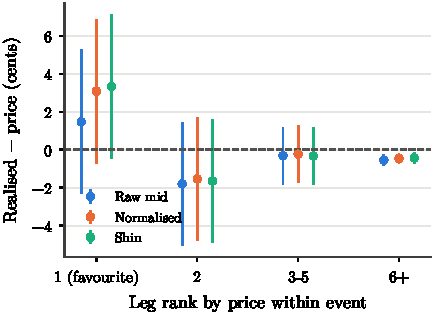
\includegraphics[width=0.55\textwidth]{figures/fig_xs_multi.pdf}
\caption{Multi-outcome events (mutually exclusive, at least three legs): realised frequency minus
price, in cents, by the leg's price rank within its event, for the raw mid, the mid normalised to
sum to one, and the Shin probability $\hat p_k(\shinz)$. 95\% confidence intervals clustered by
event.}\label{fig:xs-multi}
\end{figure}

\clearpage
